\documentclass[8pt, final,hyperref={pdfpagelabels=false}]{beamer}
\mode<presentation>{\usetheme[simple_logo]{chalmersposter}}

  \usepackage{times}
  \usepackage{amsmath,amsthm, amssymb, latexsym}
  \boldmath
  \usepackage[english]{babel}
  \usepackage{siunitx}
  \usepackage[utf8]{inputenc}
  \usepackage{graphicx}
  \usepackage{subcaption}
  \usepackage[orientation=portrait ,size=a0,scale=1.4,debug]{beamerposter}
  \usepackage[authoryear, round]{natbib}
  %%%%%%%%%%%%%%%%%%%%%%%%%%%%%%%%%%%%%%%%%%%%%%%%%%%%%%%%%%%%%%%%%%%%%%%%%%%%%%%%%5
  \title{Retrieving cloud microphysics from combined RADAR and radiometer observations}
  \author{\vspace{-1.5cm}\textbf{Simon Pfreundschuh}$^1$, Patrick Eriksson$^1$, David Duncan$^1$,
    Robin Ekelund$^1$, Stuart Fox$^2$, Florian Ewald $^3$, Stefan A. Buehler$^4$, Manfred Brath$^4$}
  \def\bibfont{\scriptsize}
  \contactauthor{Simon Pfreundschuh}
  \authormail{simon.pfreundschuh@chalmers.se}
  \institute{$^1$Chalmers University of Technology, %
      $^2$Met Office, %
    $^3$Ludwig-Maximilian Univiersität München, %
    $^4$Universität Hamburg}
  \date{2019-02-18}

  \setbeamerfont{institute in headline}{series = \mdseries, size = \normalsize}

  %%%%%%%%%%%%%%%%%%%%%%%%%%%%%%%%%%%%%%%%%%%%%%%%%%%%%%%%%%%%%%%%%%%%%%%%%%%%%%%%%5
  \begin{document}
  \begin{frame}
    \vspace{-3.5cm}
    \begin{columns}[t]
      \begin{column}{.48\linewidth}

%%%%%%%%%%%%%%%%%%%%%%%%%%%%%%%%%%%%%%%%%%%%%%%%%%%%%%%%%%%%%%%%%%%%%%%%%%%%%%%%
% Abstract
%%%%%%%%%%%%%%%%%%%%%%%%%%%%%%%%%%%%%%%%%%%%%%%%%%%%%%%%%%%%%%%%%%%%%%%%%%%%%%%%
          
        \begin{block}{Abstract}

          \begin{itemize}
          \item A novel combined retrieval approach combining microwave RADAR with
            passive microwave and sub-millimeter radiometer observations is applied
            to  retrieve cloud microphysics.
          \item The retrieval is performed for three ice-habit types to investigate
                whether observations constrain particle shape.
          \end{itemize}

        \end{block}

%%%%%%%%%%%%%%%%%%%%%%%%%%%%%%%%%%%%%%%%%%%%%%%%%%%%%%%%%%%%%%%%%%%%%%%%%%%%%%%%
% Joint flight campaign
%%%%%%%%%%%%%%%%%%%%%%%%%%%%%%%%%%%%%%%%%%%%%%%%%%%%%%%%%%%%%%%%%%%%%%%%%%%%%%%%
          
        \begin{block}{Joint flight}

          \begin{minipage}[t]{0.6\textwidth}
            \vspace{0pt}
            \begin{itemize}
            \item Joint flight of HALO, FALCON and FAAM aircraft as part of the
              North Atlantic Waveguide and Downstream Impact Experiment (NAWDEX)
              on 14th of October 2016
            \end{itemize}
            \begin{minipage}[b]{0.4\textwidth}
              \vspace{0pt}
              \rule{0pt}{5cm}
            \end{minipage}\hfill%
            \begin{minipage}[b]{0.5\textwidth}
              \vspace{1cm}
              \begin{figure}
              \caption{Flight path of the joint flight campaign  north west of Scotland.}
              \end{figure}
            \end{minipage}
          \end{minipage}%
          \begin{minipage}[t]{0.38\textwidth}
            \vspace{-2cm}
            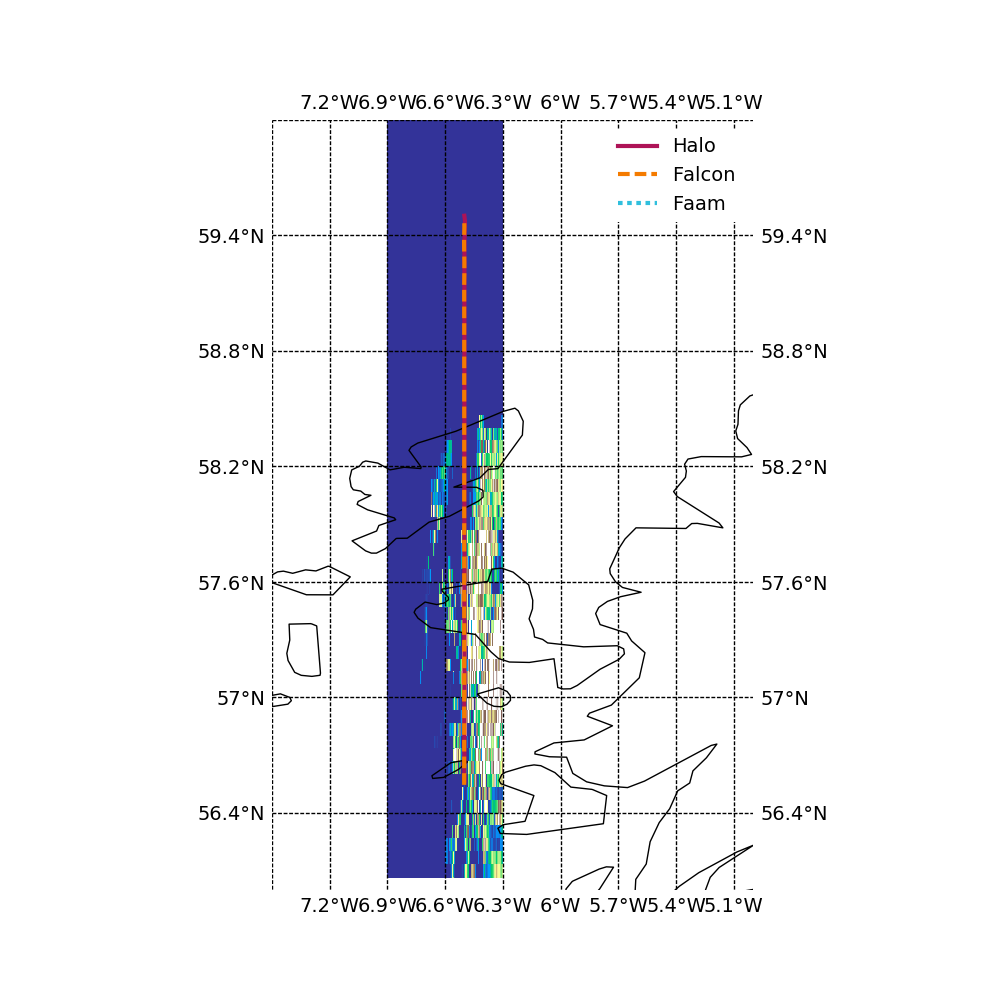
\includegraphics[width=1.0\textwidth]{../plots/flight_path.png}
          \end{minipage}%

           \textbf{Observations}

           \vspace{1.5cm}
           \centering
          \begin{tabular}{|c|c|c|c|}
            \hline
            Name & Type & Frequencies [GHz]& Reference \\
            \hline
            \hline
            HAMP RADAR & Active  & 36  & \cite{hamp}\\
            \hline
            HAMP Passive & Passive  & 27,  53, 90, 118, 183 & \cite{hamp}\\
            \hline
            ISMAR & Passive  & 118, 243, 325, 664 & \cite{ismar} \\
            \hline
          \end{tabular}

            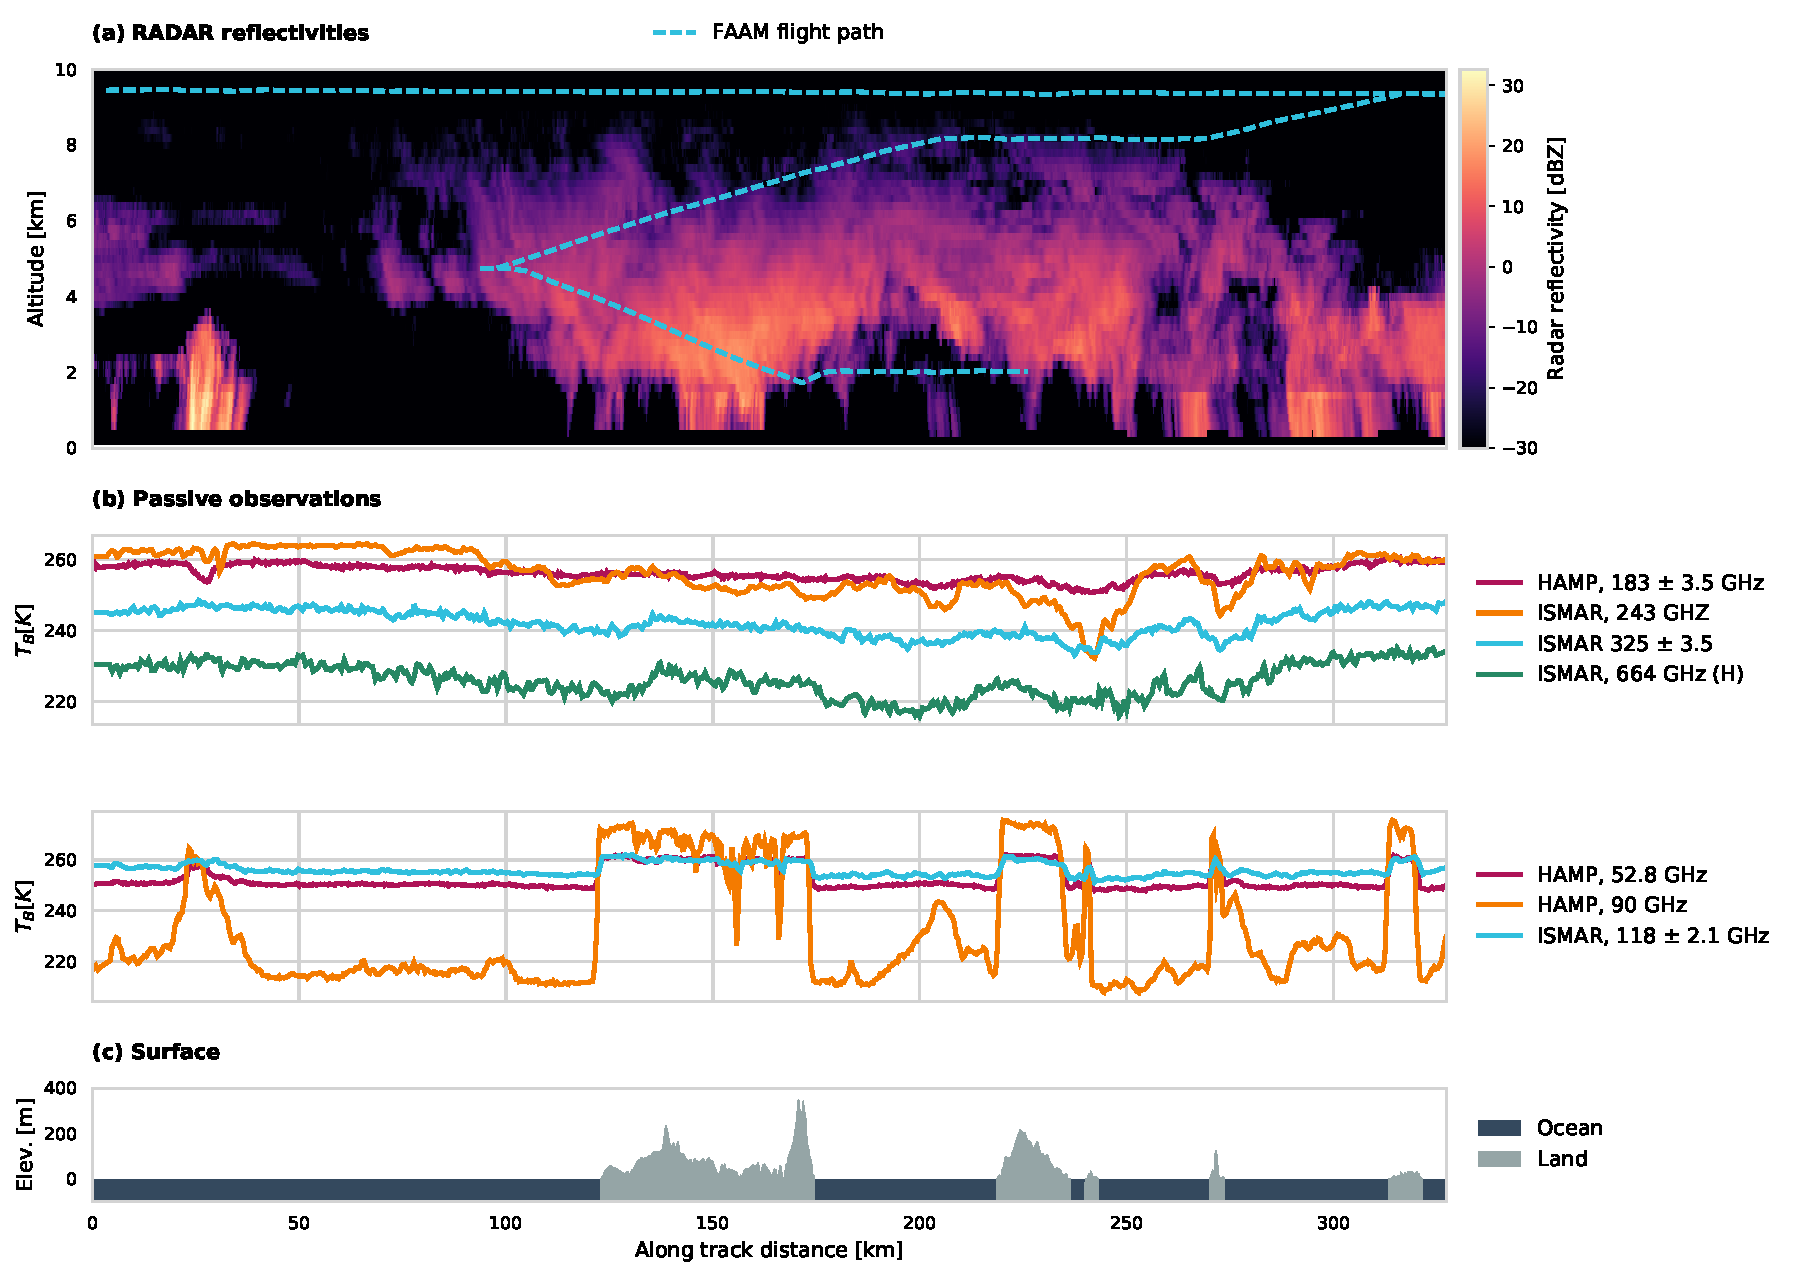
\includegraphics[width=1.0\textwidth]{../plots/observations_combined}
            \begin{figure}
            \centering
            \caption{Overview of the combined observations used in the cloud retrieval.
              Panel (a) shows the measured RADAR reflectivity. Panels (b) displays a
              selection of the micro- and sub-mm wave channels used in the retrieval.
              Panel (c) shows the surface type and surface elevation along the flight path.}
            \end{figure}
        \end{block}

%%%%%%%%%%%%%%%%%%%%%%%%%%%%%%%%%%%%%%%%%%%%%%%%%%%%%%%%%%%%%%%%%%%%%%%%%%%%%%%%
% Combined retrieval
%%%%%%%%%%%%%%%%%%%%%%%%%%%%%%%%%%%%%%%%%%%%%%%%%%%%%%%%%%%%%%%%%%%%%%%%%%%%%%%%
          
        \vspace{-2cm}
        \begin{block}{Combined cloud retrieval}

          \begin{itemize}
          \item \textbf{Method}: Optimal estimation using ARTS  \citep{arts} as forward model
          \item \textbf{Retrieval targets}: Frozen hydrometeors (1 or 2 species
            depending on settings), Liquid hydrometeors (2 species), Humidity
          \item \textbf{Microphysics}:
           \begin{itemize}
             \item Scattering properties:  ARTS SSDB \citep{arts_ssdb}
             \item Particle size distribution: Normalized gamma distribution \citep{delanoe}
%              \begin{tabular}{|c|c|c|}
%                \hline
%                Habit & $a$ & $b$ \\
%                \hline
%                \hline
%                8-column aggregate & 64.448  & 3  \\
%                \hline
%                Large plate aggregate & 0.2085 & 2.2571 \\
%                \hline
%                Large column aggregate & 0.2758 & 2.444 \\
%                \hline
%              \end{tabular}

           \end{itemize}
          \end{itemize}\\[1cm]

           \begin{figure}
             \begin{center}
             \begin{subfigure}[t]{0.3\textwidth}
               \includegraphics[width = 0.6\textwidth]{../plots/8ca}
               \vspace{0.3cm}
                \begin{small} \\$a = 64.448$, $b = 3$\end{small}
               \vspace{0.3cm}
               \caption{8-Column aggregate}
             \end{subfigure}%
             \begin{subfigure}[t]{0.3\textwidth}
               \includegraphics[width = 0.6\textwidth]{../plots/lpa}
               \vspace{0.3cm}
                \begin{small} \\$a = 0.2085$, $b = 2.2571$\end{small}
               \vspace{0.3cm}
               \caption{Large plate aggregate}
             \end{subfigure}%
             \begin{subfigure}[t]{0.32\textwidth}
               \includegraphics[width = 0.6\textwidth]{../plots/lca}
               \vspace{0.3cm}
                \begin{small} \\$a = 0.2758$, $b = 2.444$\end{small}
               \vspace{0.3cm}
               \caption{Large column aggregate}
             \end{subfigure}\hfill%
           % caption is wrong.
             \end{center}
             \caption{Ice habits and mass size relation coefficients used in the combined
               retrieval.}
           \end{figure}

        \end{block}

    \end{column}

%%%%%%%%%%%%%%%%%%%%%%%%%%%%%%%%%%%%%%%%%%%%%%%%%%%%%%%%%%%%%%%%%%%%%%%%%%%%%%%%
% Results
%%%%%%%%%%%%%%%%%%%%%%%%%%%%%%%%%%%%%%%%%%%%%%%%%%%%%%%%%%%%%%%%%%%%%%%%%%%%%%%%
          
    \begin{column}{.48\linewidth}

      \begin{block}{Retrieval results}
            \begin{figure}
            \centering
            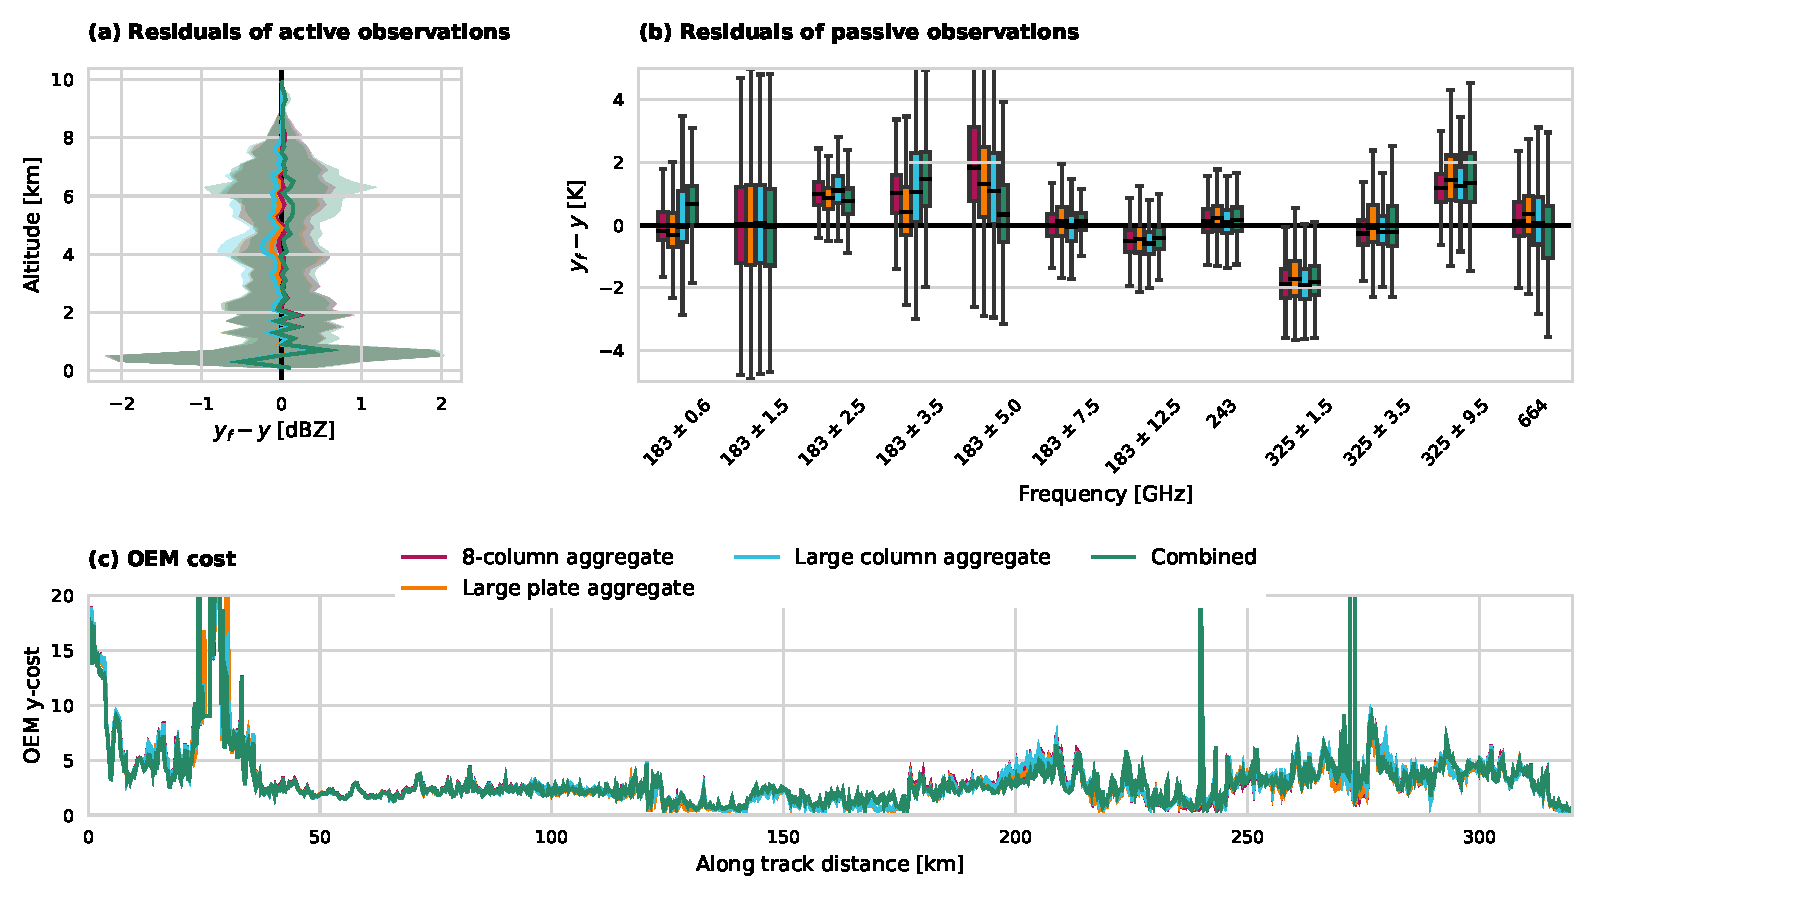
\includegraphics[width = \textwidth]{../plots/fit_overview}
            \end{figure}
            \begin{figure}
            \centering
            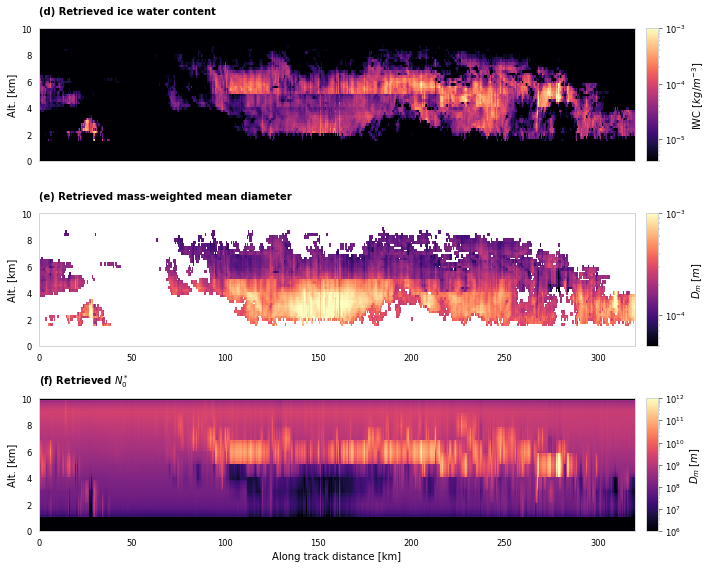
\includegraphics[width = \textwidth]{../plots/hmc}
            \caption{Panels (a) and (b) show the distributions of the residuals of
              the fitted observations. Panel (c) shows the final y-component of the
              OEM cost for the retrieved scene. Panel (d) and (e) show retrieval results
              for the large plate aggregate.}
            \end{figure}
       \end{block}

      \vspace{-1cm}

      \begin{block}{Validation}
        \begin{minipage}{0.5\textwidth}
          \begin{itemize}
            \item In-situ measurements performed during descent through cloud (c.f. Fig. 2).
            \item IWC from Nevzorov probe
          \item $D_m$ values derived from cloud imaging probes using three different
            mass-size relations.
          \end{itemize}%
          \end{minipage}%
          \begin{minipage}{0.5\textwidth}
            \begin{figure}
            \centering
            \hspace{-0.5cm}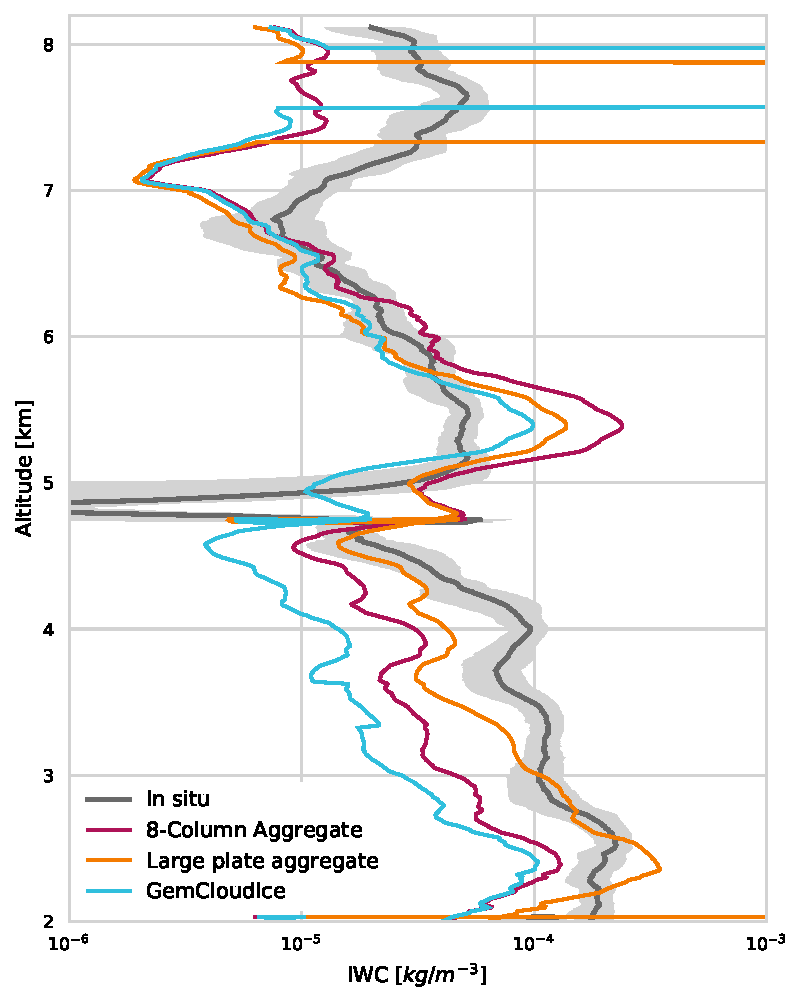
\includegraphics[width = \textwidth]{../plots/iwc_in_situ}
            \end{figure}
            \end{minipage}
      \end{block}
      \vspace{-0.5cm}

      \begin{block}{Conclusions}
        \begin{itemize}
          \item Good fit to observations indicates consistency of forward model over
            microwave and sub-mm domain.
          \item Independence of retrieval fit from habit may indicate lack of shape
               information in the combined observations.
          \item Retrieved microphysical properties show reasonable agreement with
            in-situ measurements but miss ice at the top of the cloud.
         \end{itemize}
      \end{block}
      \vspace{-0.5cm}

      \begin{block}{Acknowledgements}
        \begin{scriptsize}
          \begin{itemize}
          \item ISMAR has been jointly funded by the Met Office and the European Space Agency under the “Cloud and Precipitation Airborne Radiometer” project. The authors would also like to thank the crew and personnel involved in the NAWDEX campaign. The BAe-146 research aircraft is operated by Airtask and Avalon and managed by the Facility for Airborne Atmospheric Measurements (FAAM), which is jointly funded by the Met Office and Natural Environment Research Council (NERC). Flight B984 was funded by the European Space Agency.
            \item HAMP RADAR and radiometer data taken from \cite{halo}.
            \end{itemize}
          \end{scriptsize}
      \end{block}
      \vspace{-1cm}
      \begin{block}{References}
        \bibliographystyle{abbrvnat}
        \setcitestyle{authoryear,open={((},close={))}}
        \bibliography{literature}
      \end{block}

    \end{column}
   \end{columns}
  \end{frame}
\end{document}
